\myNewSlide
\section*{Reasons phylogenetic inference might be wrong}
\Large
\begin{compactenum}
    \item {\em Systematic error} -- Our inference method might not be sophisticated enough
    \item \underline{{\em Random error}} -- We might not have enough data --  we are misled by sampling error.
\end{compactenum}

\myNewSlide
\begin{picture}(0,0)(0,0)
      \put(-60,-280){\makebox(0,0)[l]{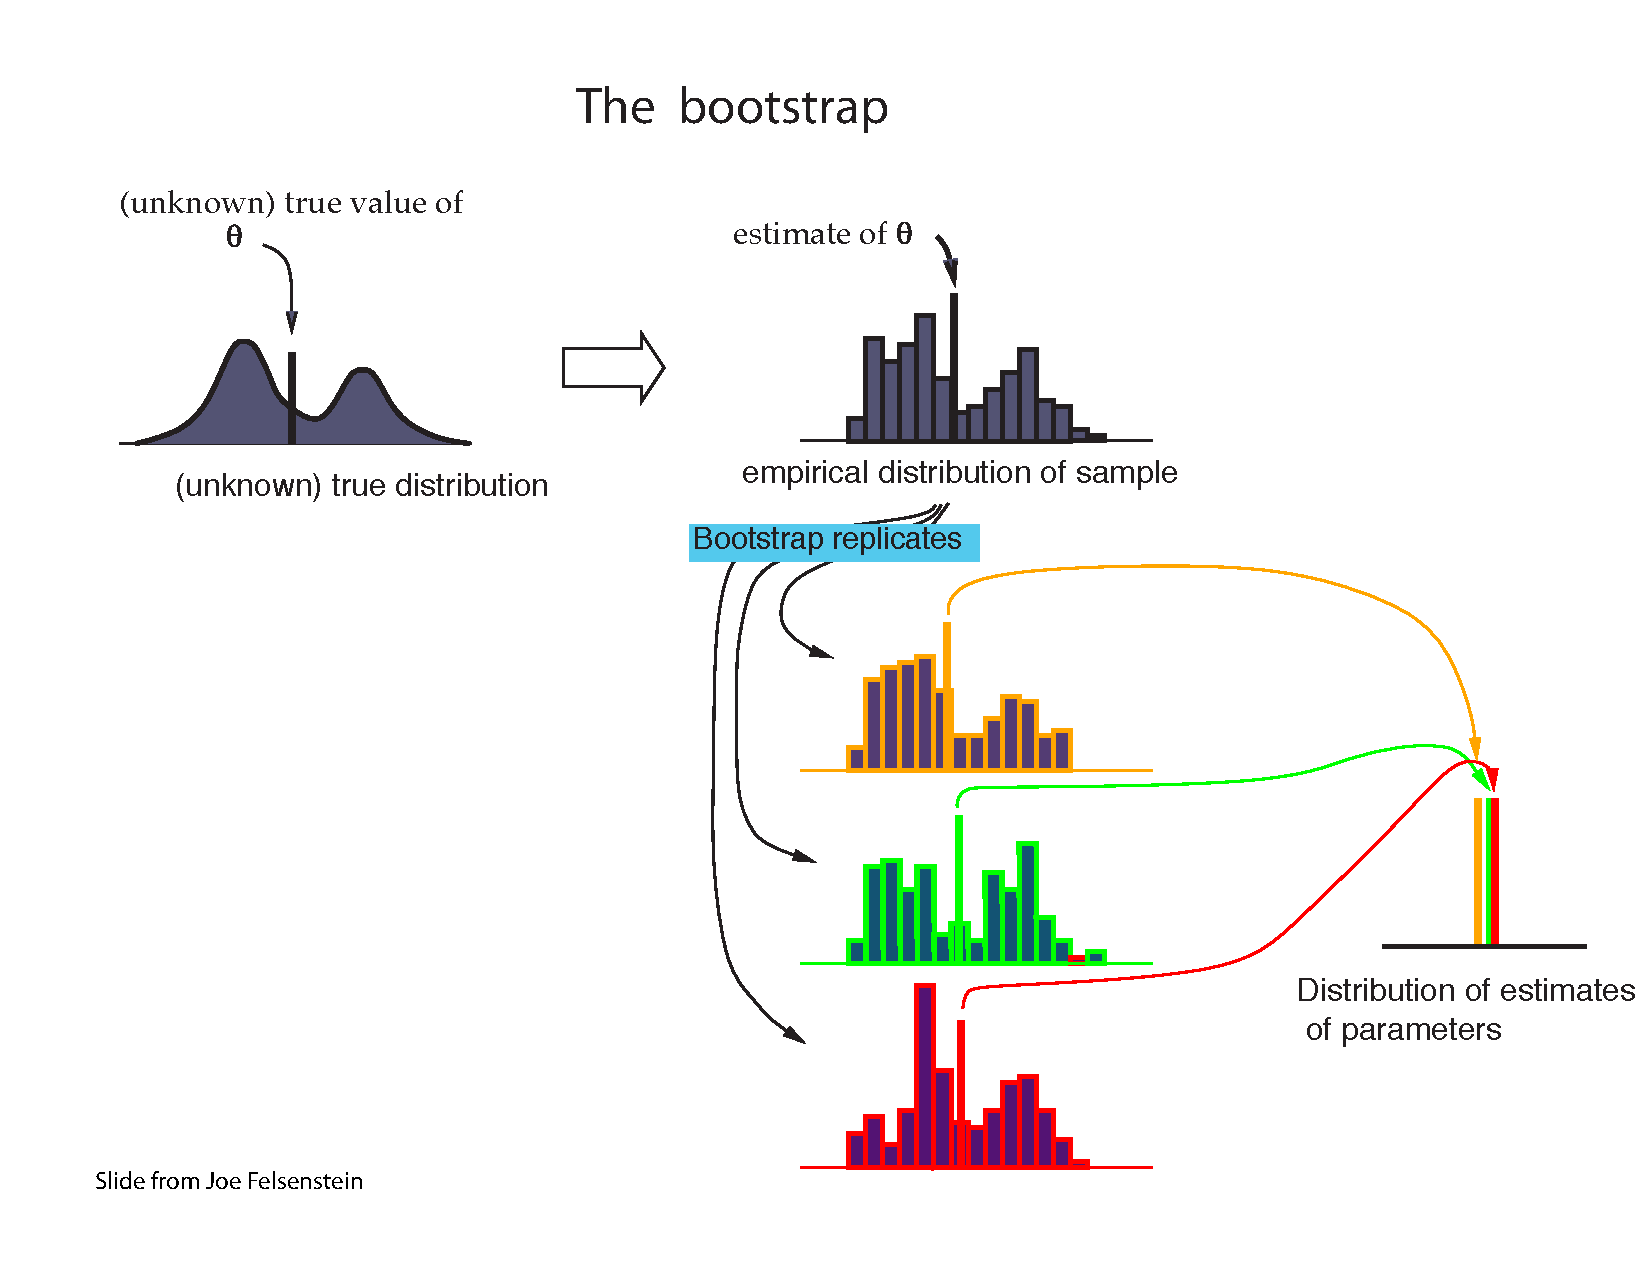
\includegraphics[scale=1.2]{../newimages/JoeFelsBootFig1.pdf}}}
      \put(0,-716){\makebox(0,0)[l]{
\includegraphics[scale=2]{../newimages/whitepage.pdf}}}
\end{picture}

\myNewSlide
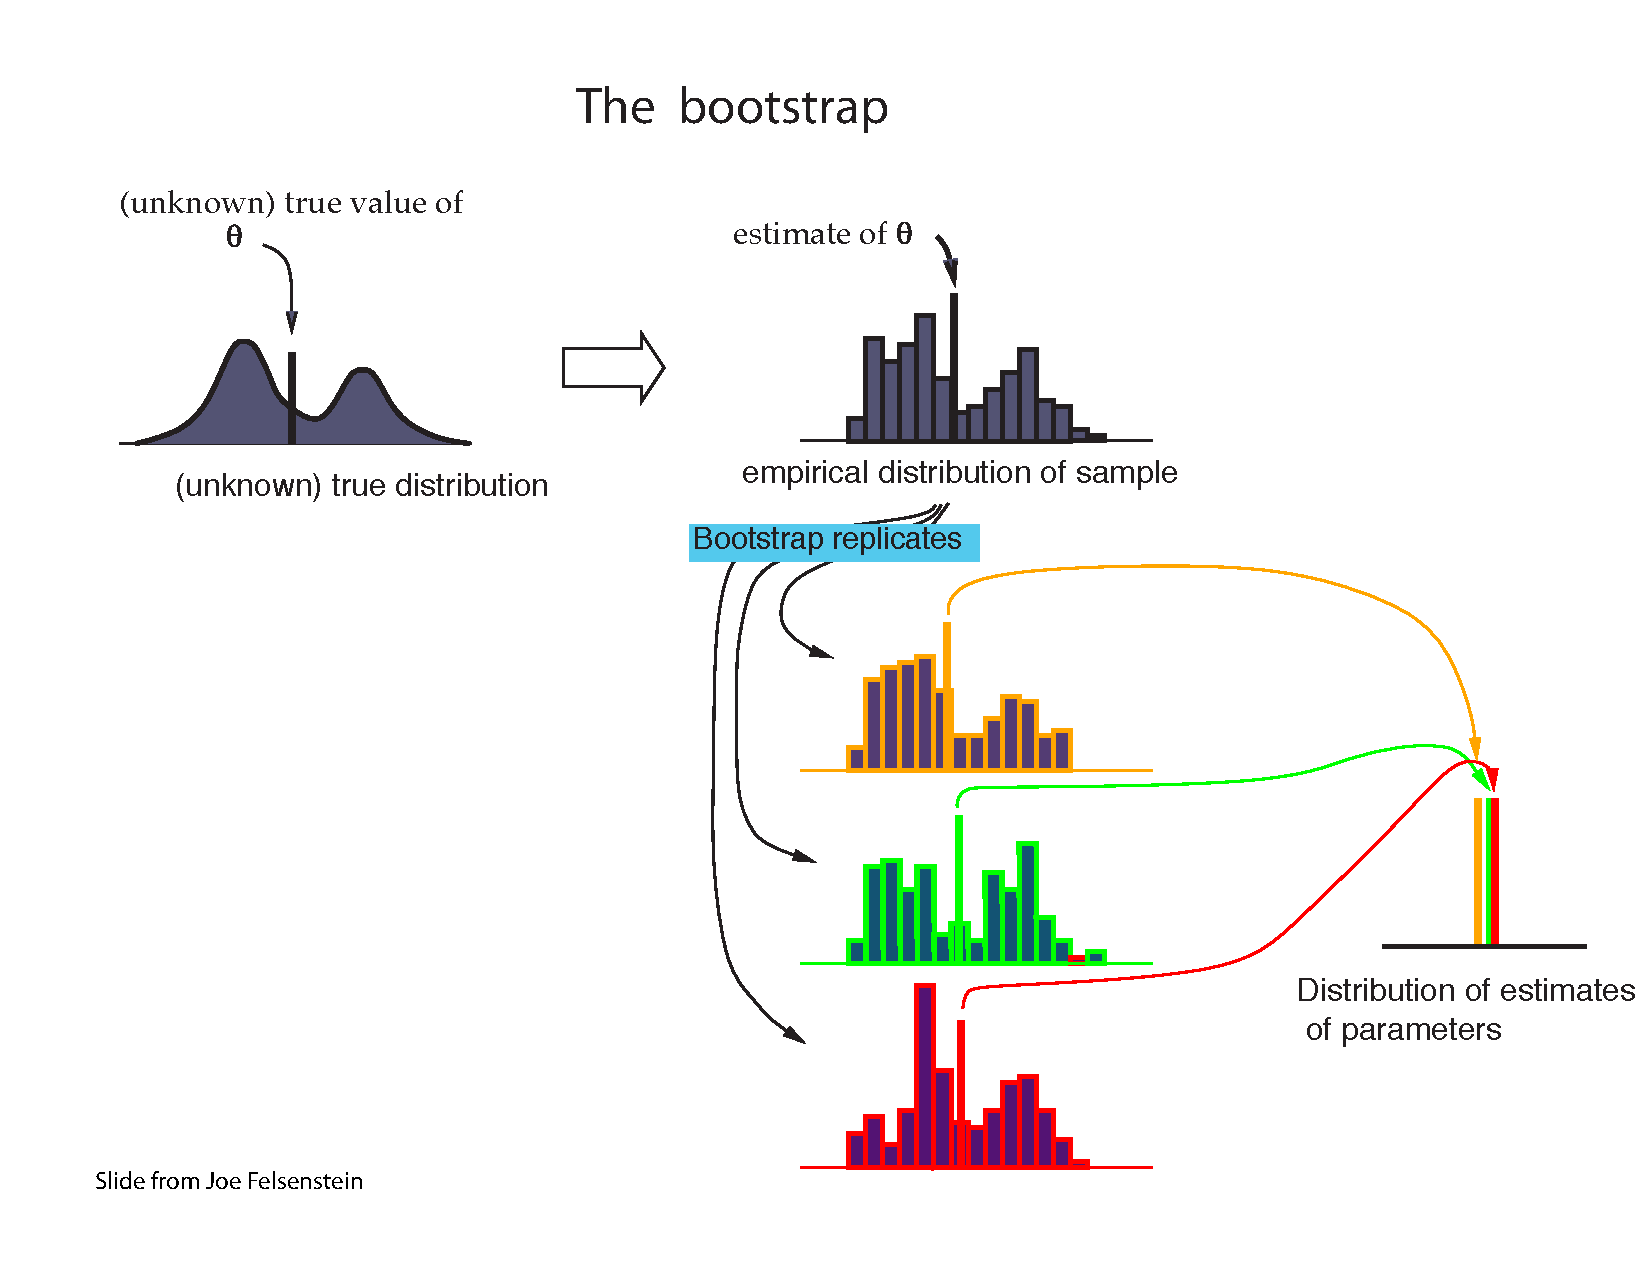
\includepdf[pages={1}]{../newimages/JoeFelsBootFig1.pdf} 

\myNewSlide
\begin{picture}(0,0)(0,0)
      \put(-70,-316){\makebox(0,0)[l]{
\includegraphics[scale=2]{../newimages/greypage.pdf}}}
      \put(-40,-200){\makebox(0,0)[l]{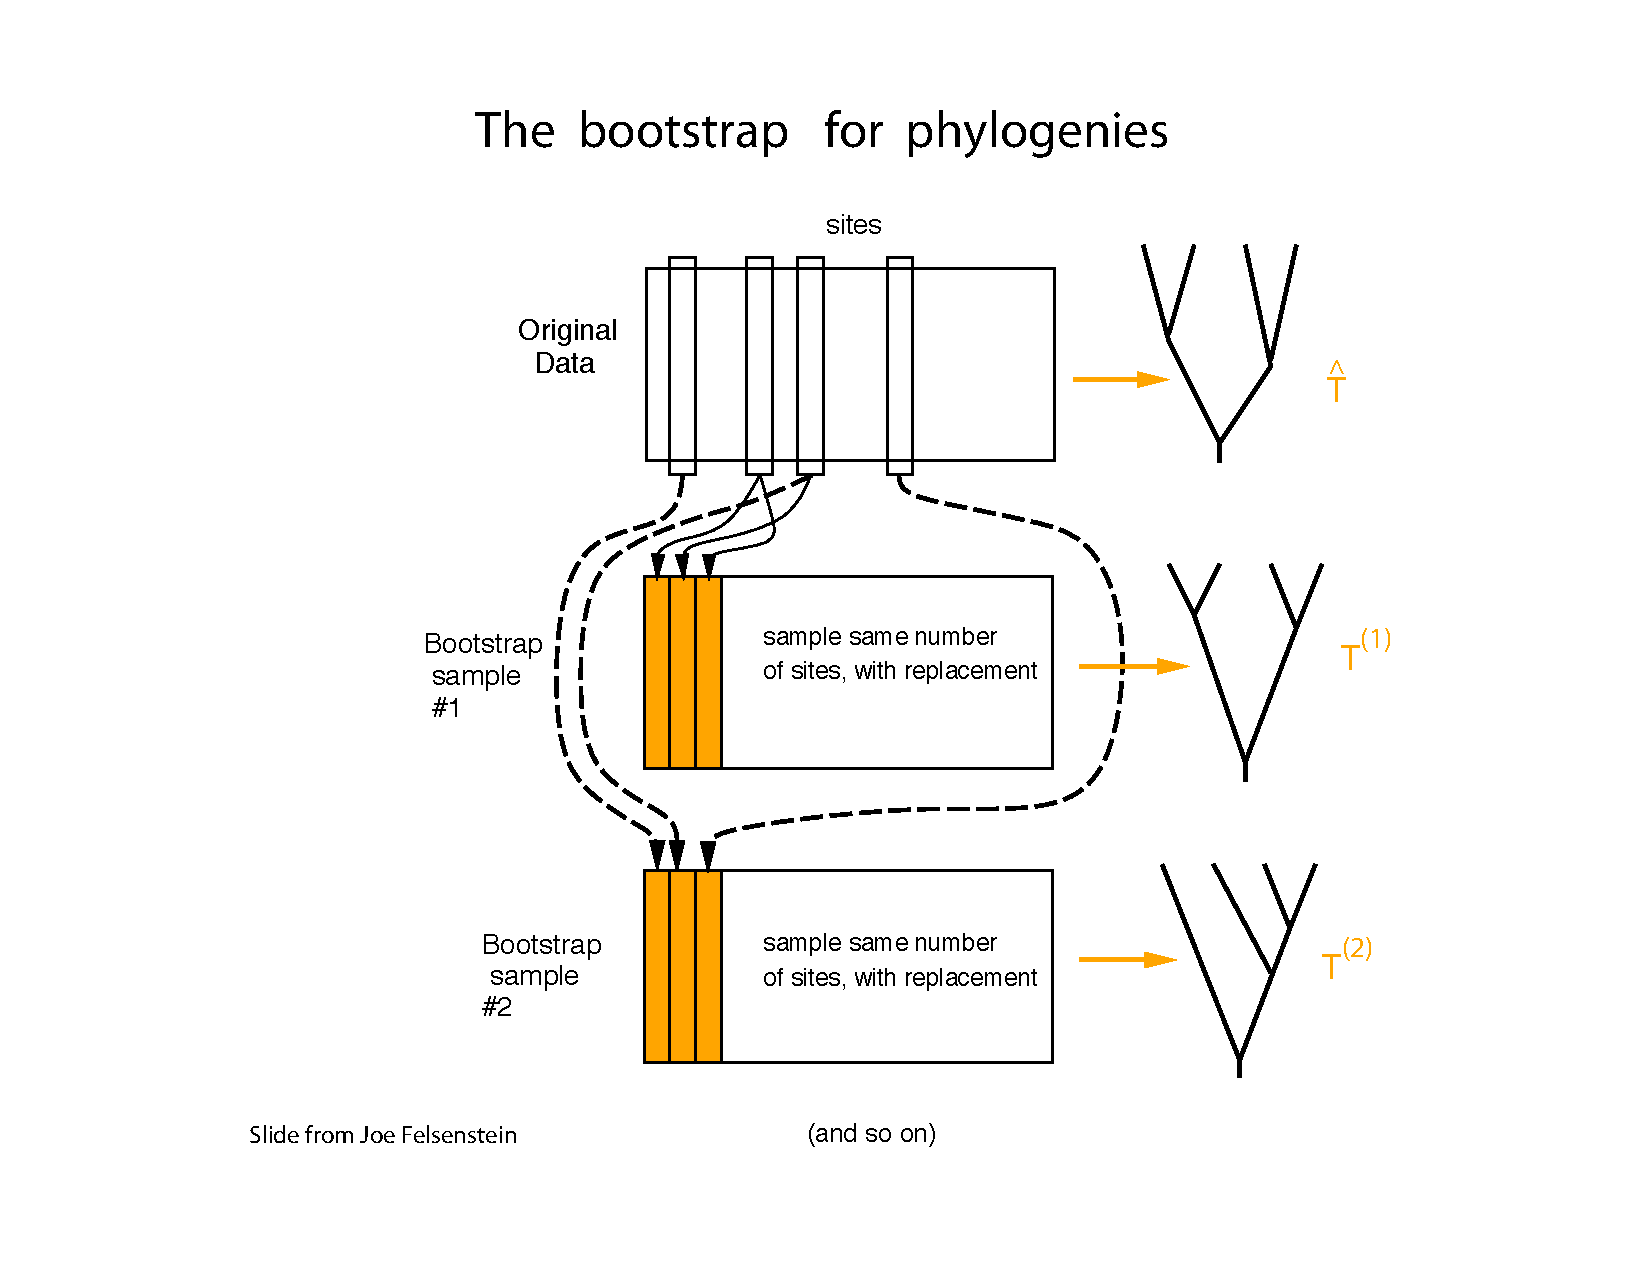
\includegraphics[scale=1.0]{../newimages/JoeFelsBootFig2.pdf}}}
\end{picture}

\myNewSlide
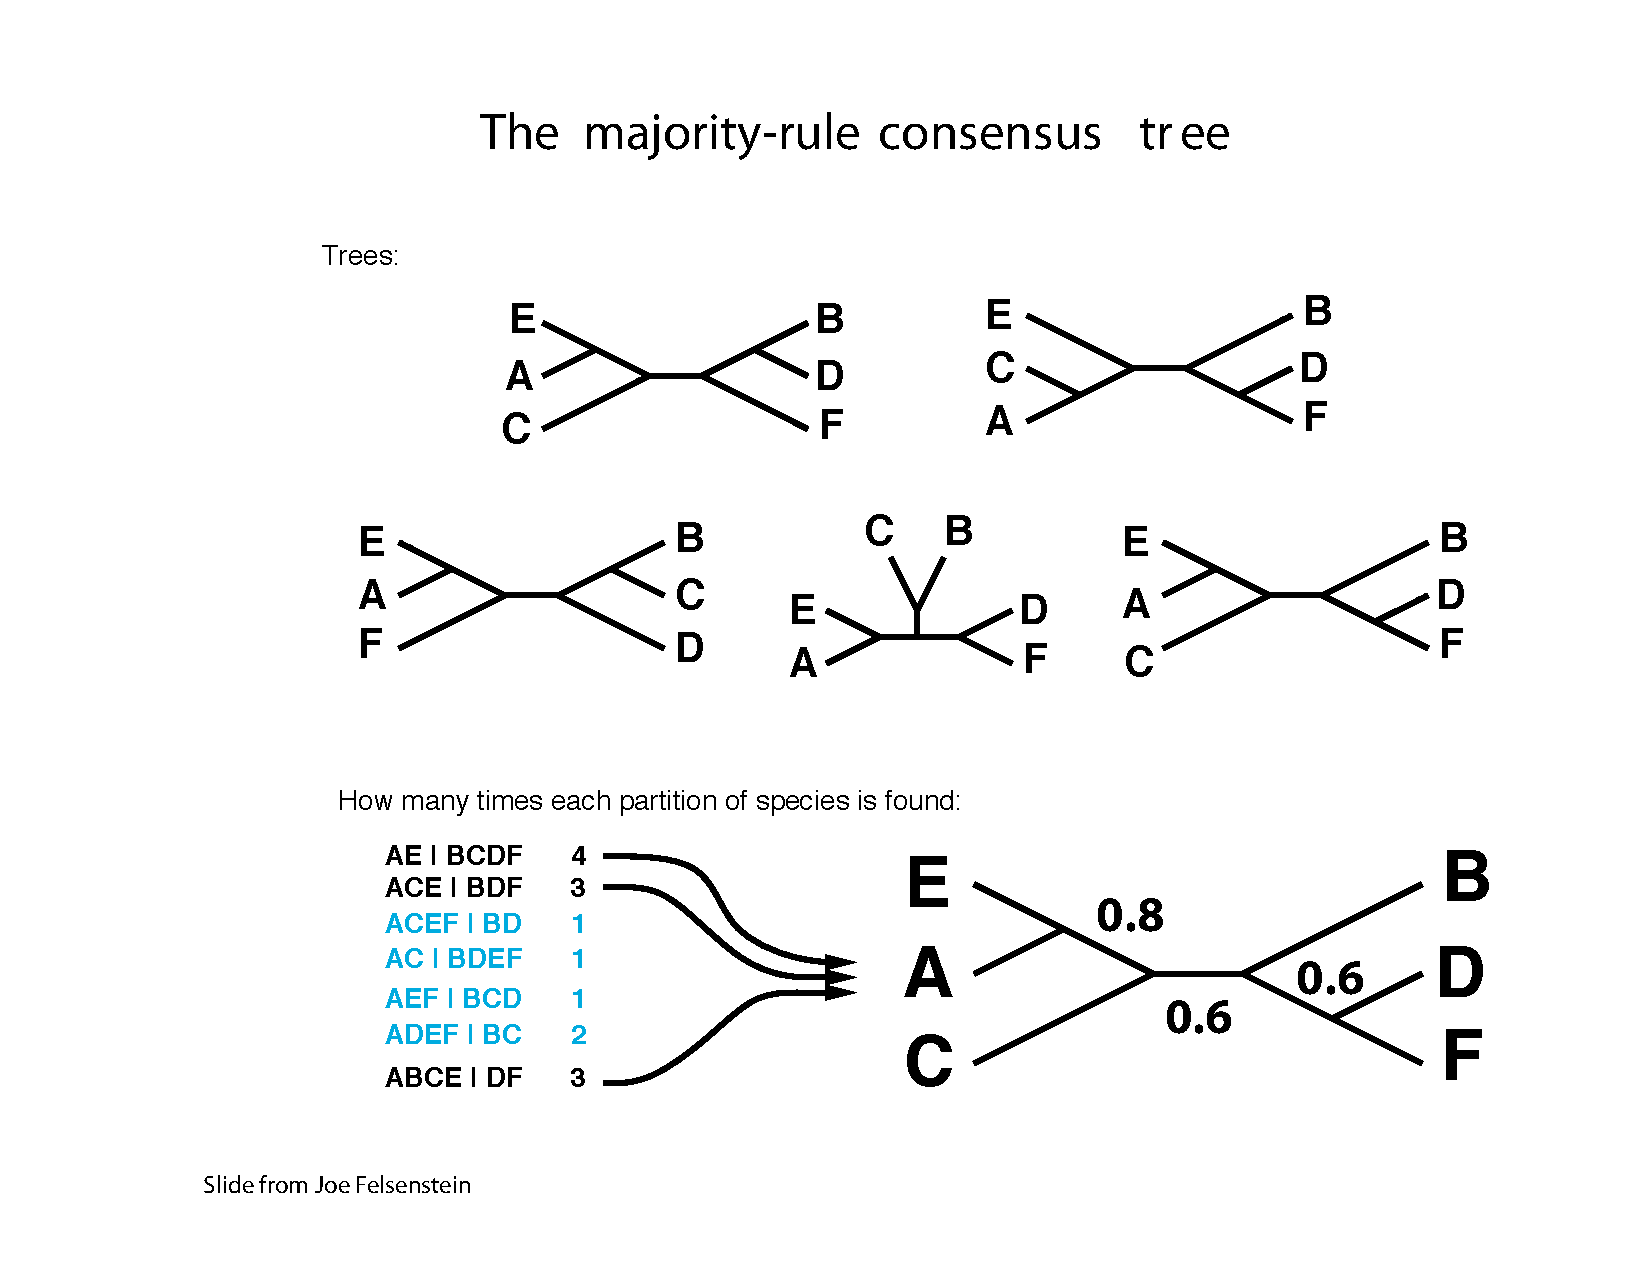
\includepdf[pages={1}]{../newimages/JoeFelsBootFig3.pdf} 



\myNewSlide
\begin{picture}(0,0)(0,0)
      \put(0,-180){\makebox(0,0)[l]{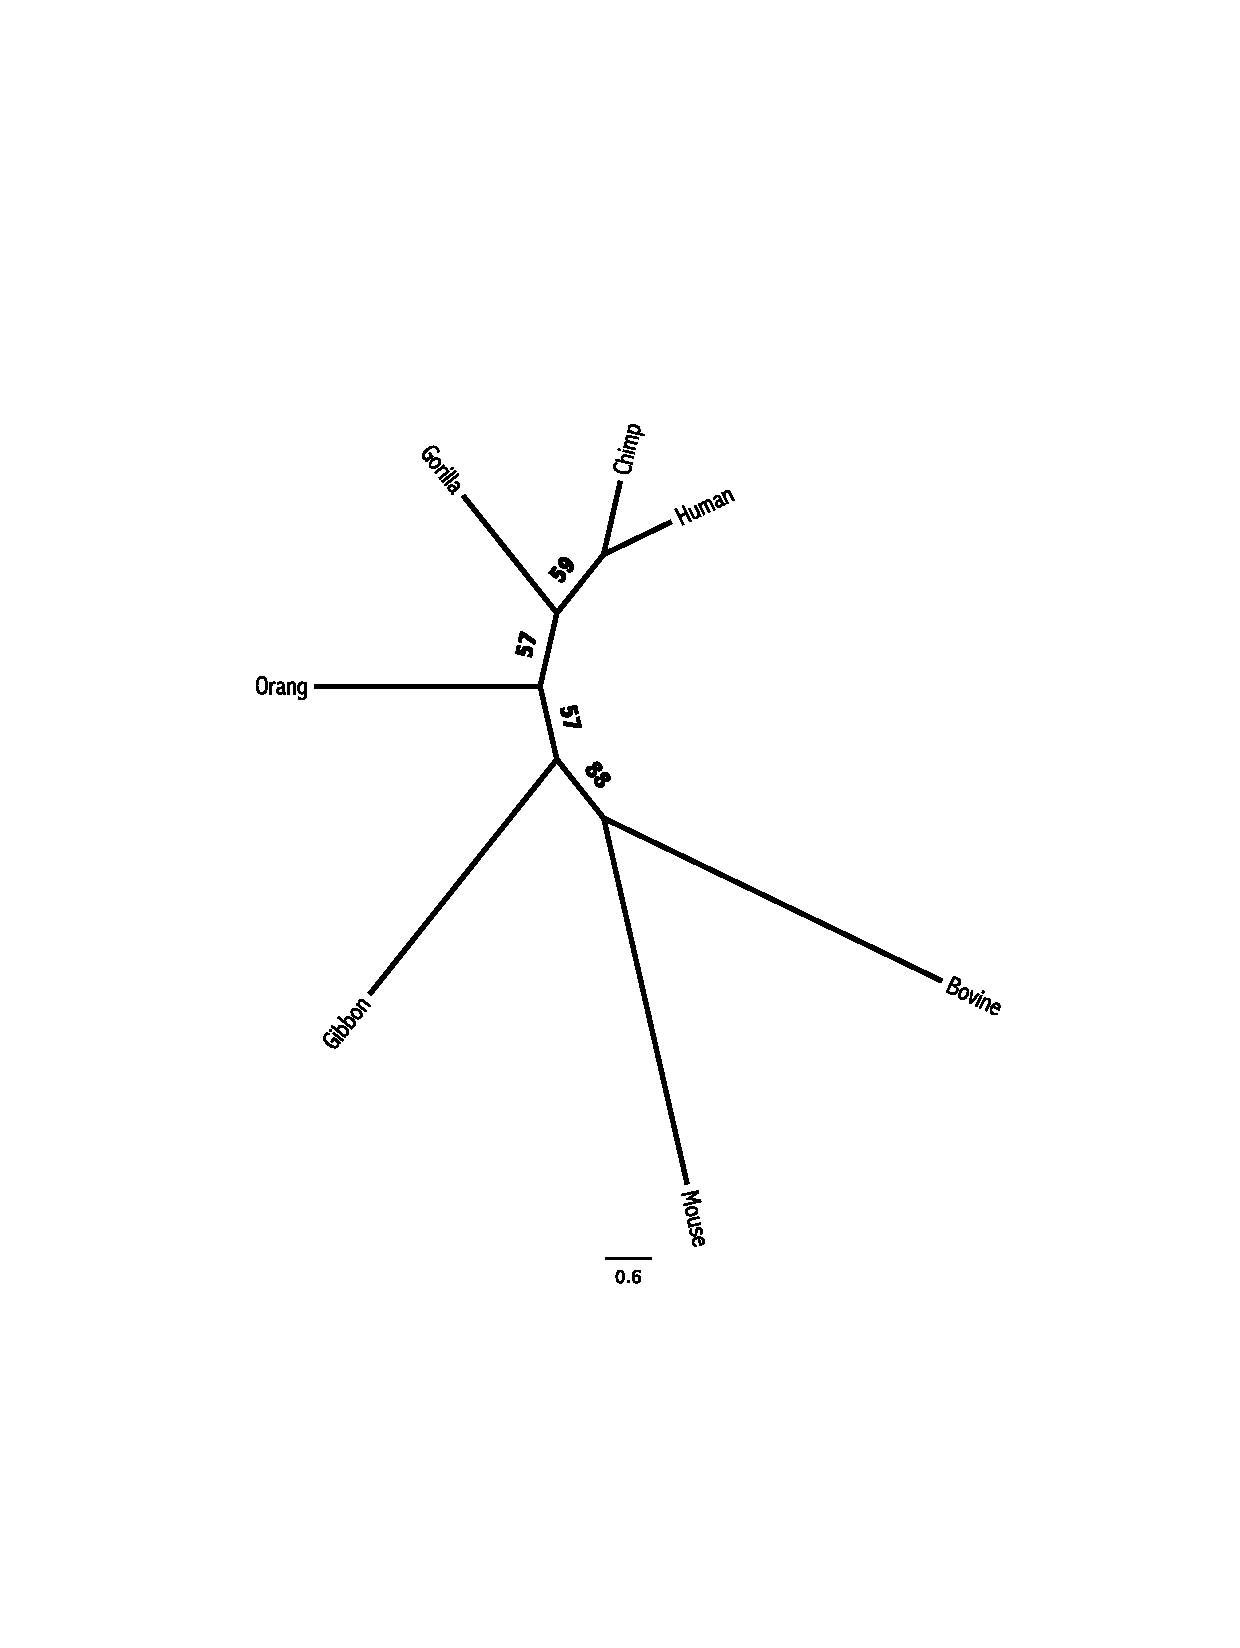
\includegraphics[scale=1.2]{../newimages/hasegawaBootFigTree.pdf}}}
      \put(0,-350){\small From Hasegawa's analysis of 232 sites D-loop}
\end{picture}

\myNewSlide
{\large
\url{http://phylo.bio.ku.edu/mephytis/boot-sample.html}

\url{http://phylo.bio.ku.edu/mephytis/parsimony.html}

\url{http://phylo.bio.ku.edu/mephytis/bootstrap.html}
}
\myNewSlide
\section*{Bootstrapping for branch support}
\large
\begin{itemize}
    \item Typically a few hundred bootstrap, pseudoreplicate datasets are produced.
    \item Less thorough searching is faster, but will usually artificially lower bootstrap proportions (BP). However, \citet{AnisimovaGDDG2011} report that RAxML's rapid bootstrap algorithm may inflate BP.
    \item ``Rogue'' taxa can lower support for many splits -- you do not have to use the majority-rule consensus tree to summarize bootstrap confidence statements.
\end{itemize}





\myNewSlide
\Large
Bootstrap proportions have been characterized as providing:
\begin{compactitem}
    \item a measure of repeatability,
    \item an estimate of the probability that the tree is correct (and bootstrapping has been criticized as being too conservative in this context),
    \item the P-value for a tree or clade
\end{compactitem}



\myNewSlide
\section*{Frequentist hypothesis testing: coin flipping example}
$N=100$ and $h=60$\\
Can we reject the fair coin hypothesis? $H_0:\Pr(\mbox{heads}) = 0.5$

The ``recipe'' is:
\begin{compactenum}
    \item Formulate null ($H_0$) and alternative ($H_A$) hypotheses.
    \item Choose an acceptable Type-I error rate (significance level)
    \item Choose a test statistic: $f_H$= fraction of heads in sample. $f_H=0.6$
    \item Characterize the null distribution of the test statistic 
    \item Calculate the $P$-value: The probability of a test statistic value more extreme than $f_H$ arising {\em even if $H_0$  is true}.
    \item Reject $H_0$ if $P$-value is $\leq$ your Type I error rate.
\end{compactenum}

\myNewSlide
\begin{picture}(500,0)(0,0)
      \put(0,-190){\makebox(0,0)[l]{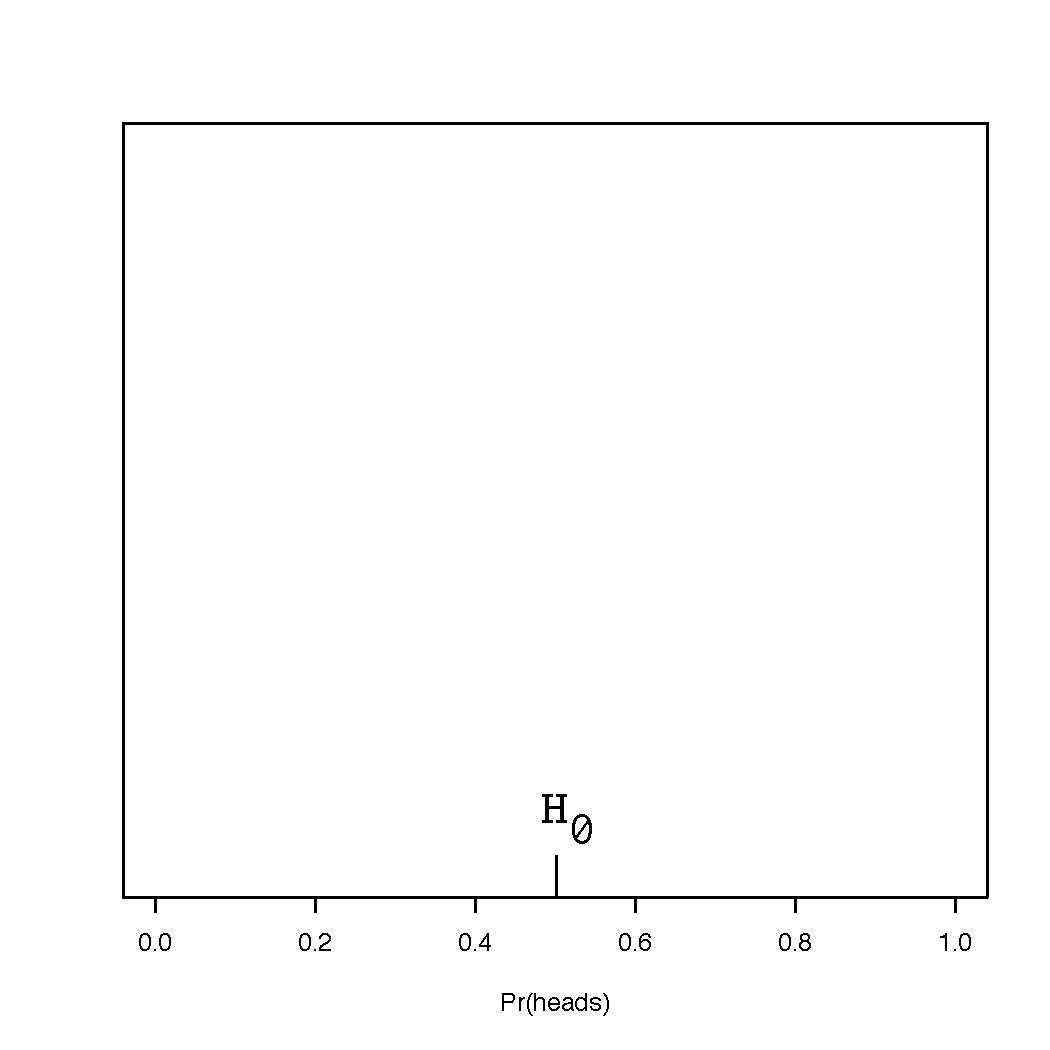
\includegraphics[scale=1.0]{../newimages/coin_axes.pdf}}}
\end{picture}

\myNewSlide
\begin{picture}(500,0)(0,0)
      \put(0,-190){\makebox(0,0)[l]{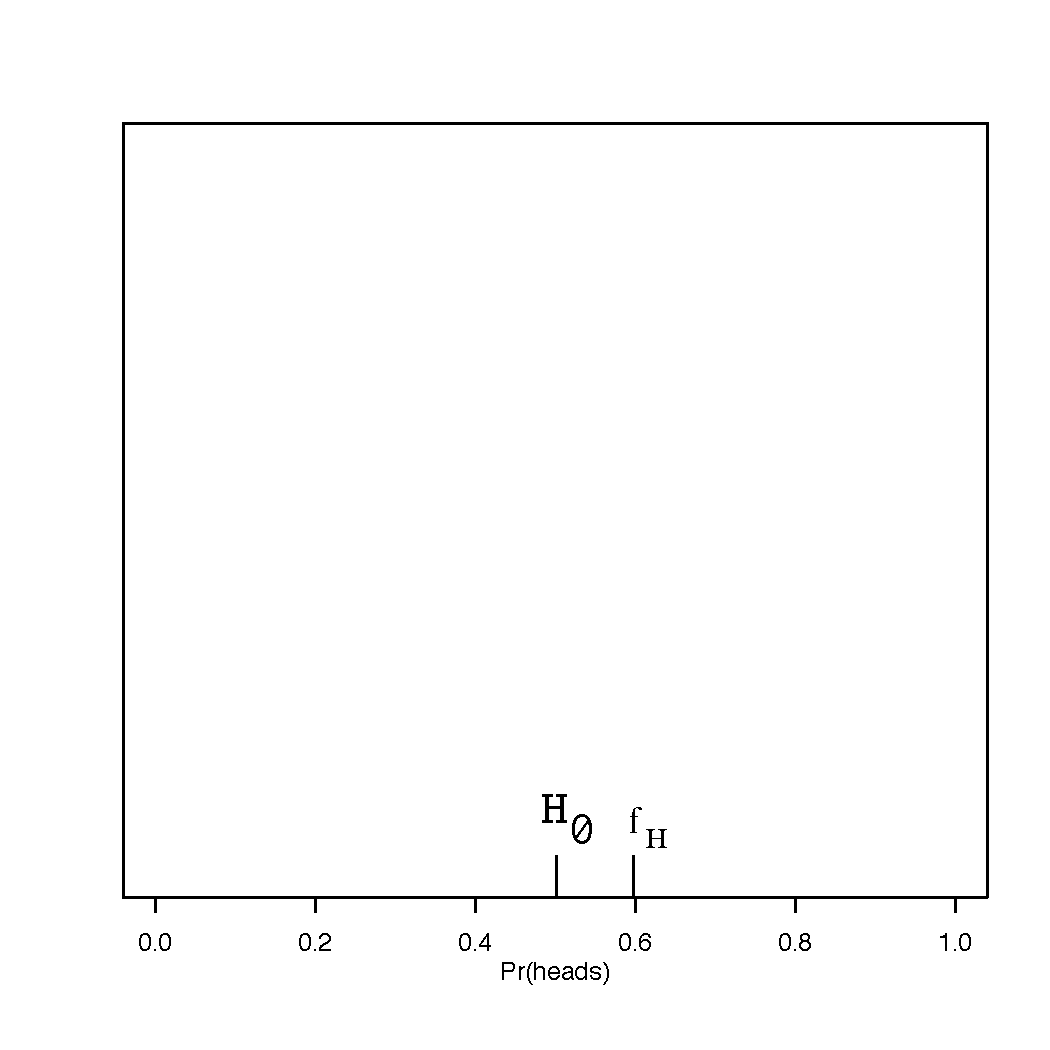
\includegraphics[scale=1.0]{../newimages/coin_axes_data.pdf}}}
\end{picture}

\myNewSlide
\section*{Null distribution}
\begin{picture}(500,0)(0,0)
      \put(0,-190){\makebox(0,0)[l]{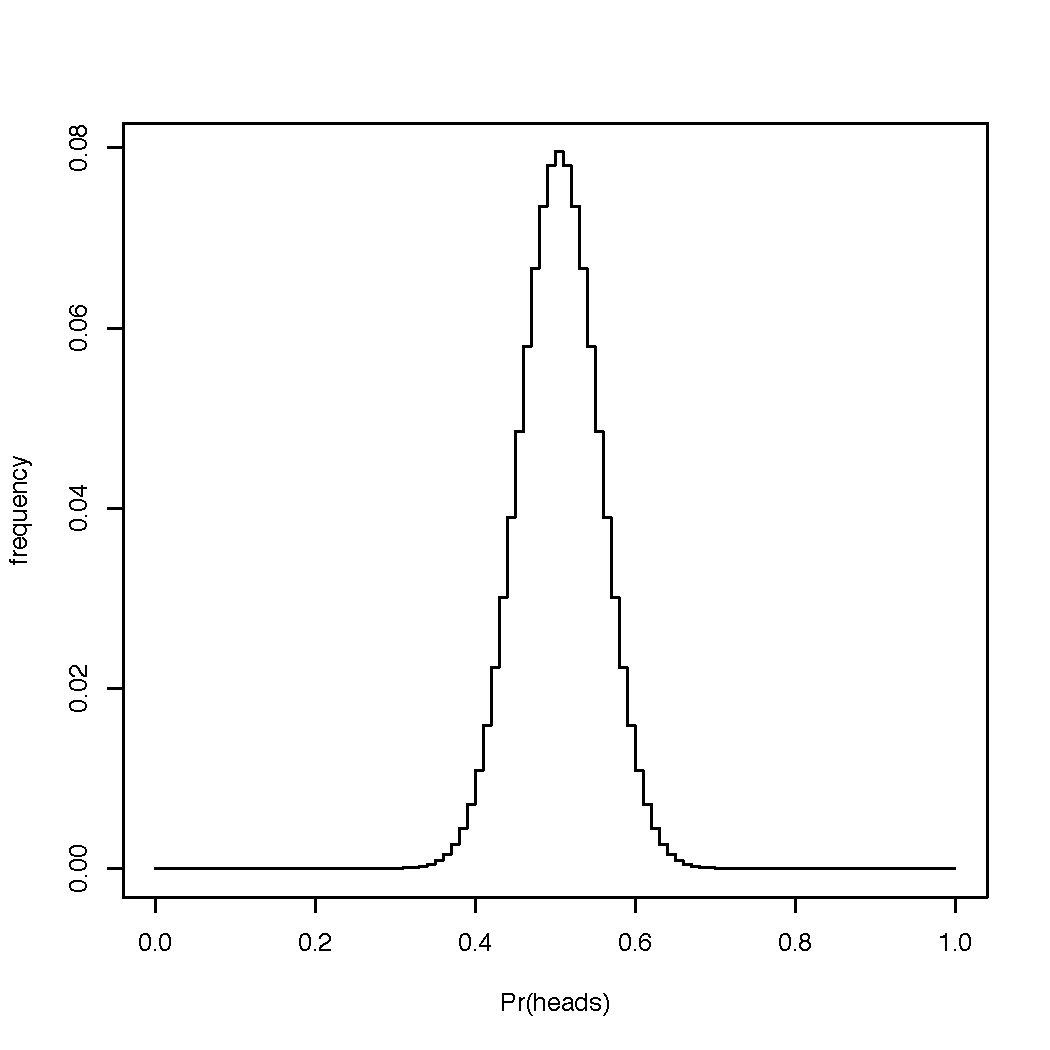
\includegraphics[scale=1.0]{../newimages/coin_wo_tails.pdf}}}
\end{picture}

\myNewSlide
\begin{picture}(500,0)(0,0)
      \put(0,-190){\makebox(0,0)[l]{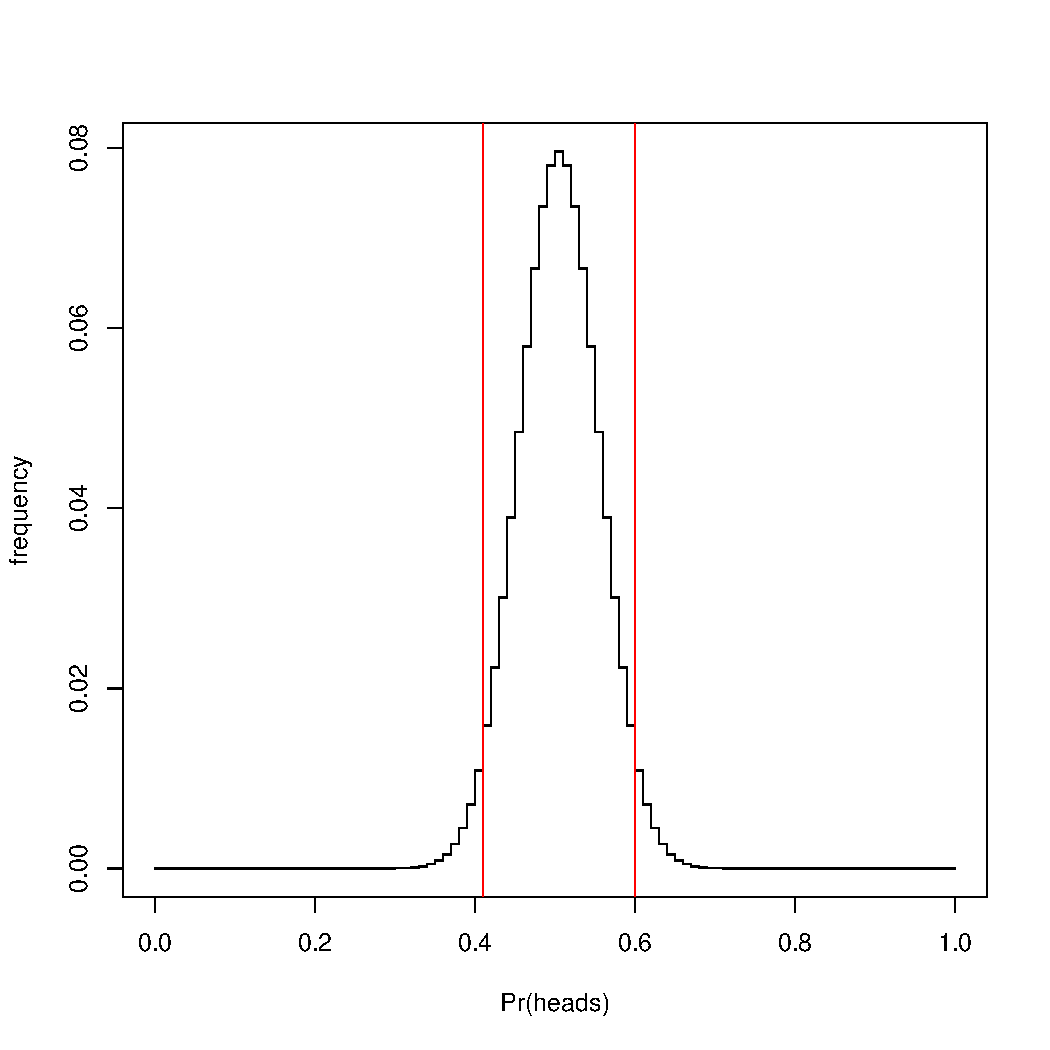
\includegraphics[scale=1.0]{../newimages/coin_w_tails.pdf}}}
      \put(0,-450){$P$-value $\approx$ 0.058}
\end{picture}

\myNewSlide
Making similar plots for tree inference is hard.

\begin{itemize}
    \item Our parameter space is trees and branch lengths.
    \item Our data is a matrix of characters.
    \item It is hard to put these objects on the same. 
    You can do this ``pattern frequency space''. Some projections of this space are:

\end{itemize}




\myNewSlide
\section*{coin flipping}
$N=100$ and $H=60$

Can we reject the hypothesis of a fair coin?

We can use simulation to generate the null distribution (we could actually use the binomial distribution to analytically solve this one)...

\myNewSlide

\begin{picture}(0,0)(0,0)
    \put(-10,-250){\makebox(0,0)[l]{\includegraphics[scale=1.0]{/home/mtholder/Documents/ku_teaching/BIOL-848-2013/images/nullhist.pdf}}}
    \put(150,-250){\color{red} P-value $\approx$ 0.029 }
\end{picture}

\myNewSlide
We discussed how bootstrapping gives us a sense of the variability ofour estimate

It can also give a tail probability for $\Pr(f_H^{(boot)} \leq 0.5)$

Amazingly (for many applications):
$$ \Pr(\hat{f}_H \geq 0.6 \mid \mbox{null is true}) \approx \Pr(f_H^{(boot)} \leq 0.5)$$

In other words, the $P$-value is approximate by the fraction of bootstrap replicates consistent with the null.
\myNewSlide

\begin{picture}(0,0)(0,0)
    \put(-60,-250){\makebox(0,0)[l]{\includegraphics[scale=1.0]{/home/mtholder/Documents/ku_teaching/BIOL-848-2013/images/boothist.pdf}}}
    \put(30,-220){\color{red}$ \Pr(p^{(boot)} \leq 0.5)\approx$ 0.027 }
    \put(30,-265){\color{red}$ BP = \mbox{frac.~of } p^{(boot)} \geq 0.5$}
    \put(30,-310){\color{red}$ BP \approx 0.973$}
    \put(30,-345){\color{red}$ P\mbox{-value} \approx 1-BP$}
\end{picture}

\myNewSlide
\begin{picture}(-0,0)(-0,0)
    \put(60,00){\makebox(30,-150)[l]{\includegraphics[scale=0.5]{/home/mtholder/Documents/ku_teaching/BIOL-848-2013/images/nullhist.pdf}}}
    \put(60,-260){\makebox(30,-150)[l]{\includegraphics[scale=0.5]{/home/mtholder/Documents/ku_teaching/BIOL-848-2013/images/boothist.pdf}}}
\end{picture}







\myNewSlide
\begin{itemize}
    \item When you decide between trees, the boundaries between tree hypotheses can be curved 
    \item When the boundary of the hypothesis space is curved, 1 - BP can be a poor approximation of the $P$-value. -- \citet{EfronHH1996}
\end{itemize}

\myNewSlide
\begin{picture}(-0,0)(-0,0)
    \put(-10,-90){\makebox(30,-150)[l]{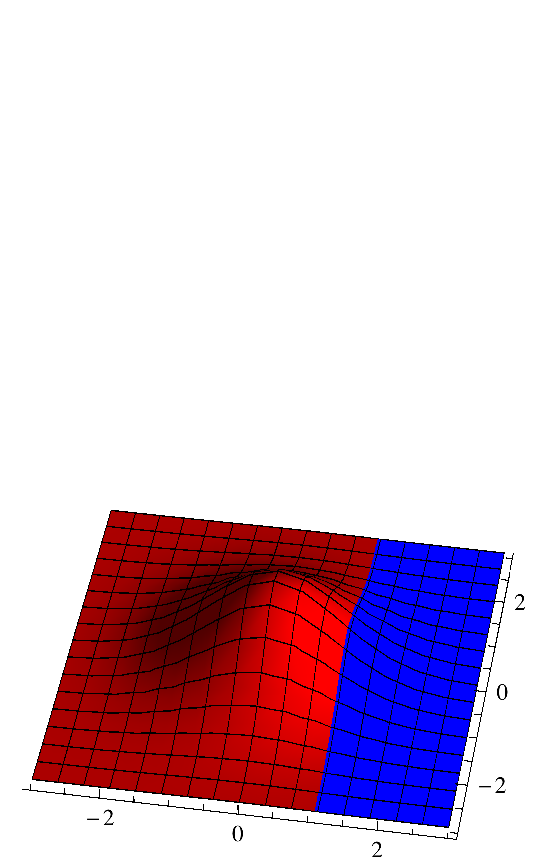
\includegraphics[scale=1.2]{../newimages/straight_p_value.pdf}}}
    \put(300,-90){\makebox(30,-150)[l]{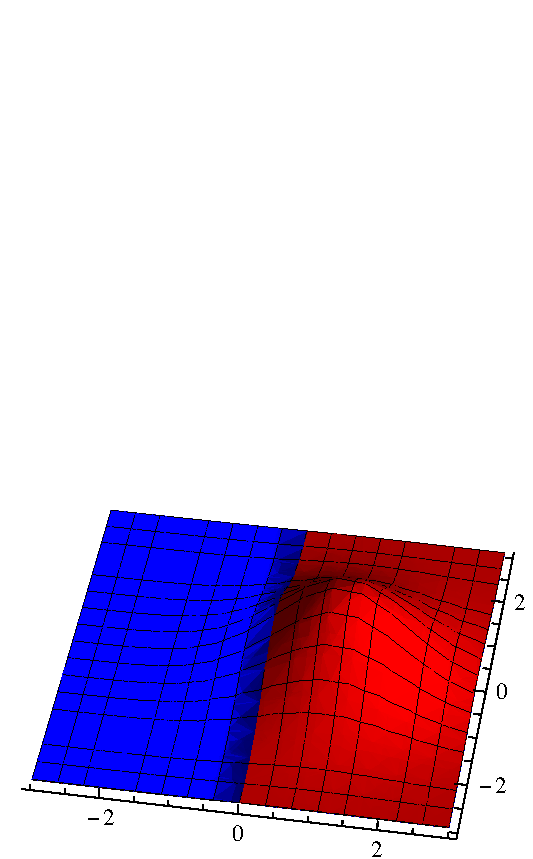
\includegraphics[scale=1.2]{../newimages/straight_boot_p_value.pdf}}}
    \put(40,0){\large In the straight border case, symmetry implies that:}
    \put(-20,-150){\large The actual $P$-value (blue region)}
    \put(420,-150){\large $\approx 1-BP$}
    \put(420,-190){\large ($1-BP$ is the blue below)}
\end{picture}

\myNewSlide

\begin{picture}(-0,0)(-0,0)
    \put(-10,-90){\makebox(30,-150)[l]{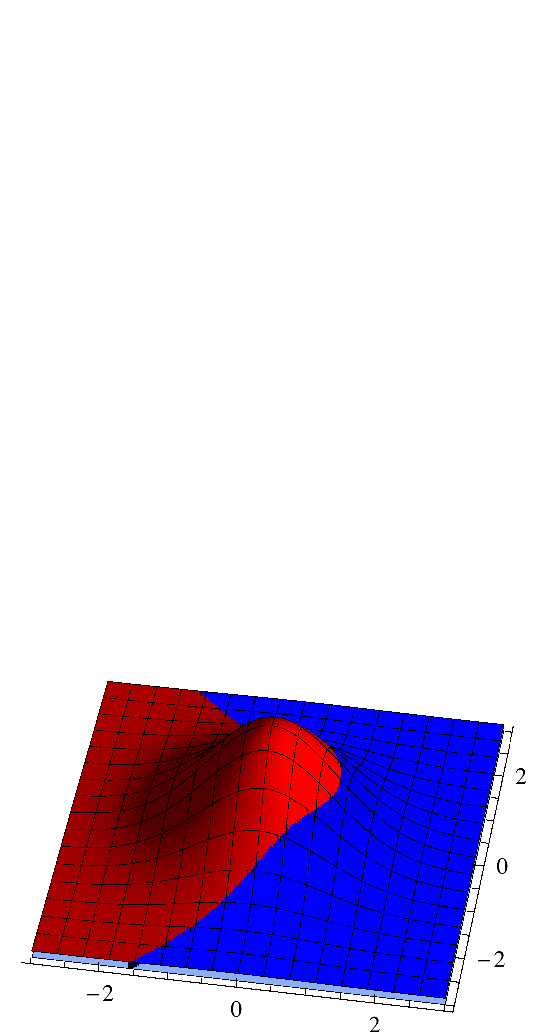
\includegraphics[scale=1.2]{../newimages/acurved_p_value.pdf}}}
    \put(300,-90){\makebox(30,-150)[l]{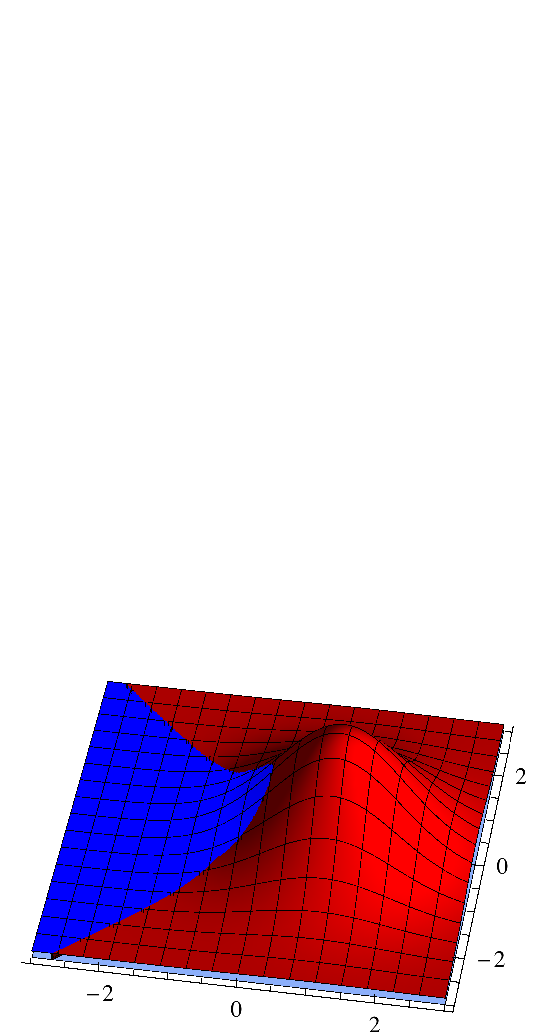
\includegraphics[scale=1.2]{../newimages/acurved_boot_p_value.pdf}}}
    \put(40,0){\large In the curved border case, the symmetry breaks down:}
    \put(-20,-150){\large The actual $P$-value (blue region)}
    \put(420,-150){\large $\neq 1-BP$}
    \put(420,-190){\large ($1-BP$ is the blue below)}
\end{picture}

\myNewSlide
\begin{itemize}
    \item \citet{EfronHH1996}  proposed a computationally expensive multi-level bootstrap (which has not been widely used).
    \item \citet{Shimodaira2002} used the same theoretical framework to devise a (more feasible) Approximately Unbiased (AU) test of topologies.
    \begin{itemize}
        \item Multiple scales of bootstrap resampling (80\% of characters, 90\%, 100\%, 110\%$\ldots$) are used to detect and correct for curvature of the boundary.
        \item Implemented in the new versions of PAUP$^{\ast}$
    \end{itemize}
\end{itemize}

\myNewSlide
\section*{\cite{Susko2010} adjusted BP -- aBP}
\large
\begin{compactitem}
    \item Susko agrees with curvature arguments of \citet{EfronHH1996} and \citet{Shimodaira2002}, {\bf but} points out that they ignore the {\bf sharp point} in parameter space around the polytomy.

    \item He correct bootstrap proportions:  $1-aBP$ accurately estimates the $P$-value.

    \item The method uses the multivariate normal distributions the based on calculations about the curvature of the {\em likelihood} surface.

    \item You need to perform a different correction when you know the candidate tree {\em a priori} versus when you are putting BP on the ML tree.

    \item BP may {\bf not} be conservative when you correct for selection bias.
\end{compactitem}

\myNewSlide
\begin{picture}(-0,0)(-0,0)
    \put(-60,-150){\makebox(30,-150)[l]{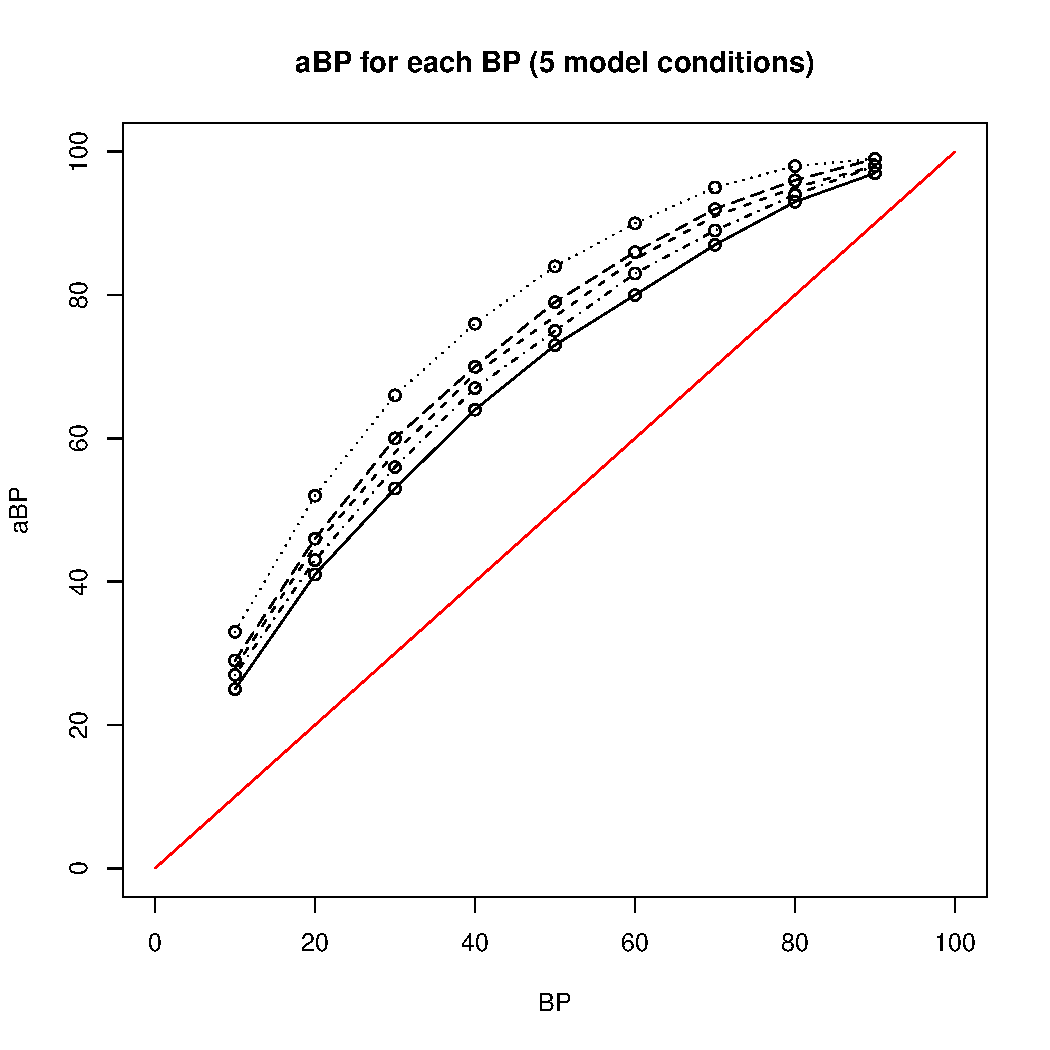
\includegraphics[scale=0.75]{../scripts/Susko2010Table3aBP.pdf}}}
    \put(300,-150){\makebox(30,-150)[l]{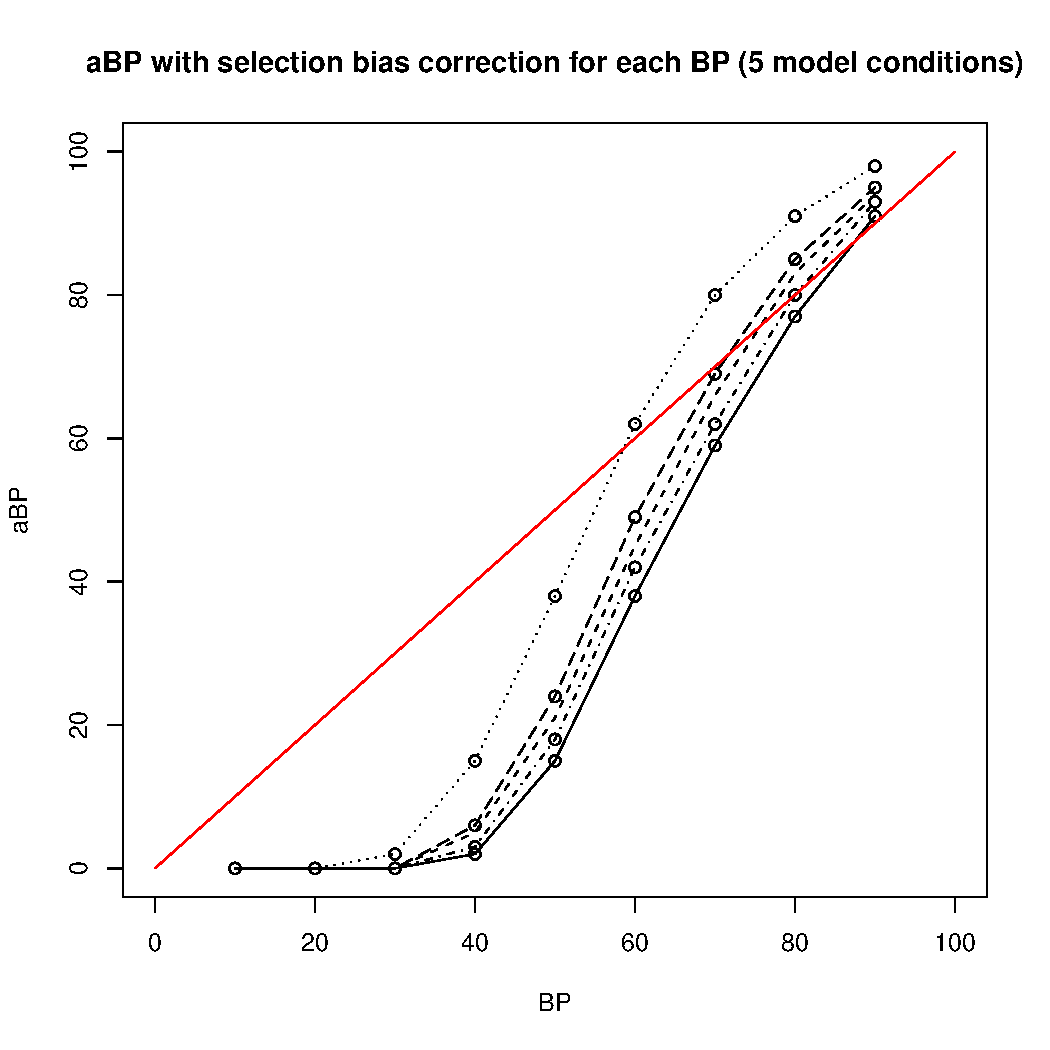
\includegraphics[scale=0.75]{../scripts/Susko2010Table3aBPMLCorrection.pdf}}}
\end{picture}

\myNewSlide
\section*{Conclusions -- bootstrapping}\large
\large
\begin{compactenum}
    \item Non-parametric bootstrapping proportions help us see which branches
    have so little support that they could be plausibly explained by sampling error.
    \item BPs are a little hard to interpret  precisely.
    \item Susko has and adjustment (``aBP``) so that $1 - aBP\approx P$-value for the hypothesis that a recovered branch is not present in the true tree. 
\end{compactitem}

